% GNUPLOT: LaTeX picture with Postscript
\begingroup
  \makeatletter
  \providecommand\color[2][]{%
    \GenericError{(gnuplot) \space\space\space\@spaces}{%
      Package color not loaded in conjunction with
      terminal option `colourtext'%
    }{See the gnuplot documentation for explanation.%
    }{Either use 'blacktext' in gnuplot or load the package
      color.sty in LaTeX.}%
    \renewcommand\color[2][]{}%
  }%
  \providecommand\includegraphics[2][]{%
    \GenericError{(gnuplot) \space\space\space\@spaces}{%
      Package graphicx or graphics not loaded%
    }{See the gnuplot documentation for explanation.%
    }{The gnuplot epslatex terminal needs graphicx.sty or graphics.sty.}%
    \renewcommand\includegraphics[2][]{}%
  }%
  \providecommand\rotatebox[2]{#2}%
  \@ifundefined{ifGPcolor}{%
    \newif\ifGPcolor
    \GPcolorfalse
  }{}%
  \@ifundefined{ifGPblacktext}{%
    \newif\ifGPblacktext
    \GPblacktexttrue
  }{}%
  % define a \g@addto@macro without @ in the name:
  \let\gplgaddtomacro\g@addto@macro
  % define empty templates for all commands taking text:
  \gdef\gplbacktext{}%
  \gdef\gplfronttext{}%
  \makeatother
  \ifGPblacktext
    % no textcolor at all
    \def\colorrgb#1{}%
    \def\colorgray#1{}%
  \else
    % gray or color?
    \ifGPcolor
      \def\colorrgb#1{\color[rgb]{#1}}%
      \def\colorgray#1{\color[gray]{#1}}%
      \expandafter\def\csname LTw\endcsname{\color{white}}%
      \expandafter\def\csname LTb\endcsname{\color{black}}%
      \expandafter\def\csname LTa\endcsname{\color{black}}%
      \expandafter\def\csname LT0\endcsname{\color[rgb]{1,0,0}}%
      \expandafter\def\csname LT1\endcsname{\color[rgb]{0,1,0}}%
      \expandafter\def\csname LT2\endcsname{\color[rgb]{0,0,1}}%
      \expandafter\def\csname LT3\endcsname{\color[rgb]{1,0,1}}%
      \expandafter\def\csname LT4\endcsname{\color[rgb]{0,1,1}}%
      \expandafter\def\csname LT5\endcsname{\color[rgb]{1,1,0}}%
      \expandafter\def\csname LT6\endcsname{\color[rgb]{0,0,0}}%
      \expandafter\def\csname LT7\endcsname{\color[rgb]{1,0.3,0}}%
      \expandafter\def\csname LT8\endcsname{\color[rgb]{0.5,0.5,0.5}}%
    \else
      % gray
      \def\colorrgb#1{\color{black}}%
      \def\colorgray#1{\color[gray]{#1}}%
      \expandafter\def\csname LTw\endcsname{\color{white}}%
      \expandafter\def\csname LTb\endcsname{\color{black}}%
      \expandafter\def\csname LTa\endcsname{\color{black}}%
      \expandafter\def\csname LT0\endcsname{\color{black}}%
      \expandafter\def\csname LT1\endcsname{\color{black}}%
      \expandafter\def\csname LT2\endcsname{\color{black}}%
      \expandafter\def\csname LT3\endcsname{\color{black}}%
      \expandafter\def\csname LT4\endcsname{\color{black}}%
      \expandafter\def\csname LT5\endcsname{\color{black}}%
      \expandafter\def\csname LT6\endcsname{\color{black}}%
      \expandafter\def\csname LT7\endcsname{\color{black}}%
      \expandafter\def\csname LT8\endcsname{\color{black}}%
    \fi
  \fi
  \setlength{\unitlength}{0.0500bp}%
  \begin{picture}(9070.00,11338.00)%
    \gplgaddtomacro\gplbacktext{%
      \csname LTb\endcsname%
      \put(1078,2005){\makebox(0,0)[r]{\strut{}25.00}}%
      \put(1078,4173){\makebox(0,0)[r]{\strut{}30.00}}%
      \put(1078,6341){\makebox(0,0)[r]{\strut{}35.00}}%
      \put(1078,8509){\makebox(0,0)[r]{\strut{}40.00}}%
      \put(1078,10677){\makebox(0,0)[r]{\strut{}45.00}}%
      \put(1210,484){\makebox(0,0){\strut{}0.20}}%
      \put(2358,484){\makebox(0,0){\strut{}0.40}}%
      \put(3506,484){\makebox(0,0){\strut{}0.60}}%
      \put(4654,484){\makebox(0,0){\strut{}0.80}}%
      \put(5803,484){\makebox(0,0){\strut{}1.00}}%
      \put(6951,484){\makebox(0,0){\strut{}1.20}}%
      \put(8099,484){\makebox(0,0){\strut{}1.40}}%
      \put(176,5690){\rotatebox{-270}{\makebox(0,0){\strut{}$p \ [bar]$}}}%
      \put(4941,154){\makebox(0,0){\strut{}$V \ [cm^3]$}}%
      \put(4941,11007){\makebox(0,0){\strut{}Isothermennetz für Schwefelhexafluorid}}%
    }%
    \gplgaddtomacro\gplfronttext{%
      \csname LTb\endcsname%
      \put(7686,10504){\makebox(0,0)[r]{\strut{}$\vartheta \pm \Delta\vartheta = (25.9 \pm 0.1) ^\circ C$}}%
      \csname LTb\endcsname%
      \put(7686,10284){\makebox(0,0)[r]{\strut{}$\vartheta \pm \Delta\vartheta = (40.2 \pm 0.1) ^\circ C$}}%
      \csname LTb\endcsname%
      \put(7686,10064){\makebox(0,0)[r]{\strut{}$\vartheta \pm \Delta\vartheta = (43.9 \pm 0.1) ^\circ C$}}%
      \csname LTb\endcsname%
      \put(7686,9844){\makebox(0,0)[r]{\strut{}$\vartheta \pm \Delta\vartheta = (45.5 \pm 0.1) ^\circ C$}}%
      \csname LTb\endcsname%
      \put(7686,9624){\makebox(0,0)[r]{\strut{}$\vartheta \pm \Delta\vartheta = (50.2 \pm 0.1) ^\circ C$}}%
      \csname LTb\endcsname%
      \put(7686,9404){\makebox(0,0)[r]{\strut{}Isotherme für ideales Gas bei $\vartheta = 45.5 ^\circ C$}}%
    }%
    \gplbacktext
    \put(0,0){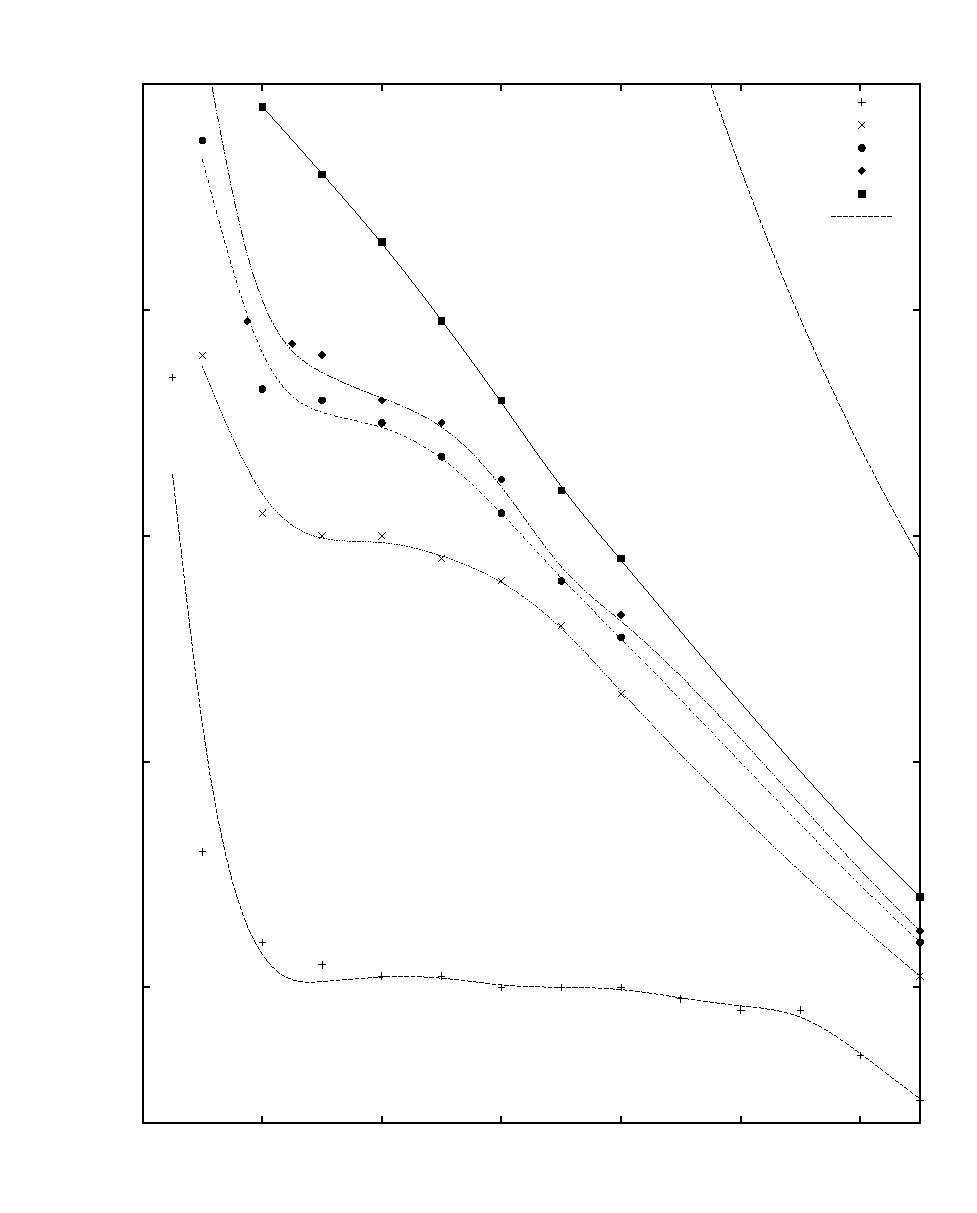
\includegraphics{diagram}}%
    \gplfronttext
  \end{picture}%
\endgroup
